\section{Quantum Double Model IV}

\subsection{Review - Flux Excitations in QD Model}
Last time, we introduced the idea that there is one type of flux excitation for every non-trivial conjugacy class $C \subseteq G$. We constructed the explicit states:
\begin{equation}
    \ket{C} = \sum_{\set{g_j}}\ket{\set{g_j}}
\end{equation}
with $\set{g_j}$ such that we have flux $C$ through plaquette $p_0$ and 1/no flux elsewhere. This is analogous to the ground state of the original Hamiltonian, except we enforce the condition where there is a nontrivial flux through one plaquette.

In arguing for this, we explained how anyons should be the unique ground state of a trapping potential. In particular, the $\ket{C}$ above is the unique ground state of:
\begin{equation}
    H = -\sum_s A(s) - \sum_{p\neq p_0}B(p) - B_C(p_0)
\end{equation}
with $B_C(p)$ defined as:
\begin{center}
    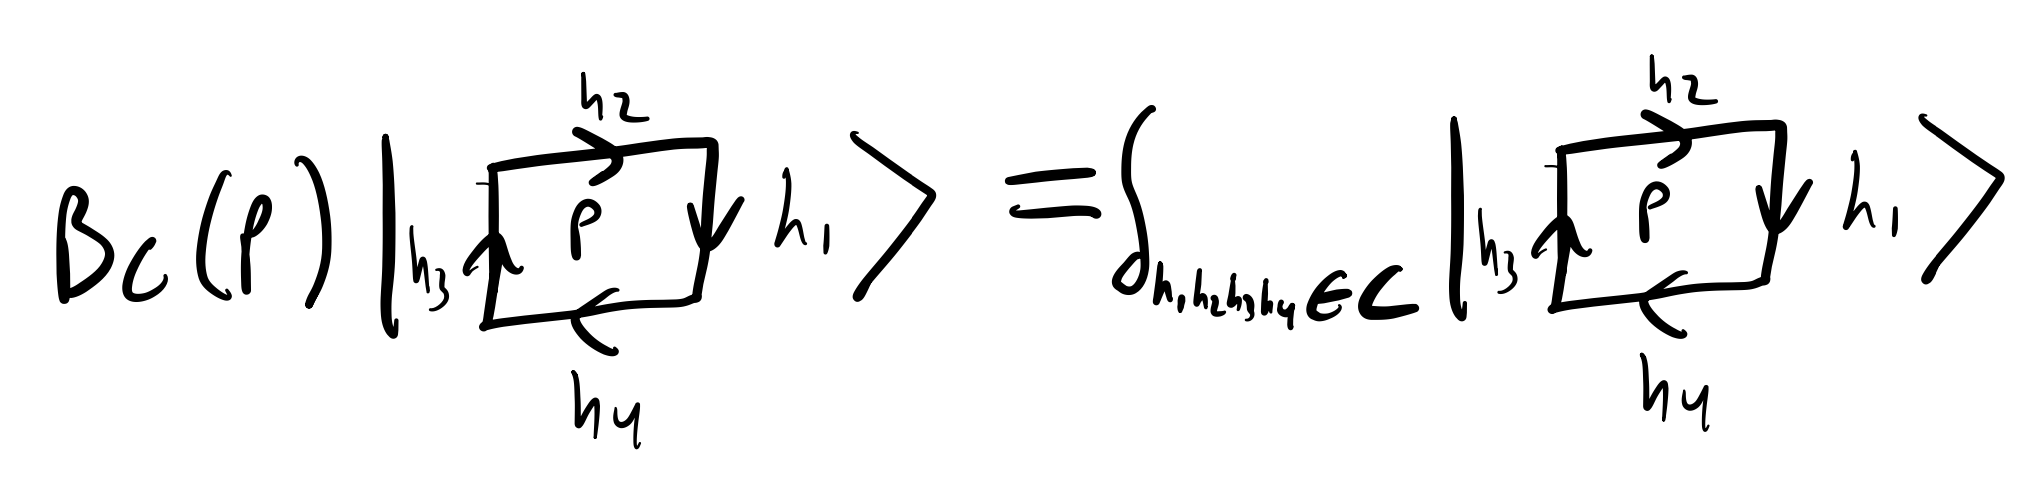
\includegraphics[scale=0.35]{Lectures/Images/lec8-Bcp.png}
\end{center}
Note that the $H$ above is a commuting projector Hamiltonian ,as $B_c(p_0)$ commutes with all the other terms. We showed that this is indeed the unique eigenstate by arguing that $B_C(\gamma)$ for a sufficiently large loop $\gamma$ around the flux can detect it, but must commute with any local operator around such a flux.

\subsection{Multiple Fluxes in QD Model}
We can easily generalize the above trapping Hamiltonian to that which traps several fluxes:
\begin{equation}
    H = -\sum_s A(s) - \sum_{p \neq p_1, \ldots p_n}B(p) - \sum_{i=1}^n B_{C_i}(p_i)
\end{equation}
\begin{center}
    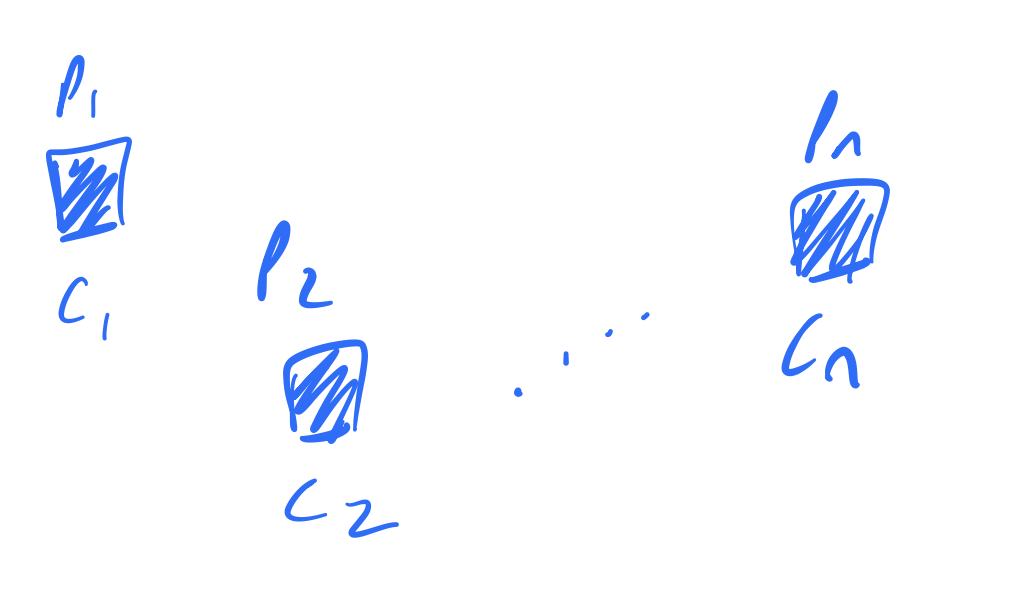
\includegraphics[scale=0.35]{Lectures/Images/lec9-multiplefluxes.png}
\end{center}

interestingly, we will find that in general $H$ has multiple degenerate ground states. To construct them, we choose different group elements in the different conjugacy classes, $g_i \in C_i$, with the constraint:

\begin{equation}
    g_1g_2 \ldots g_n = 1
\end{equation}
This constraint corresponds to ground states having trivial topological charge (and corresponds to the ability to create the ground state via a local term) - we will come back to this. We now construct the ground states in two steps. First, define the basis states:
\begin{center}
    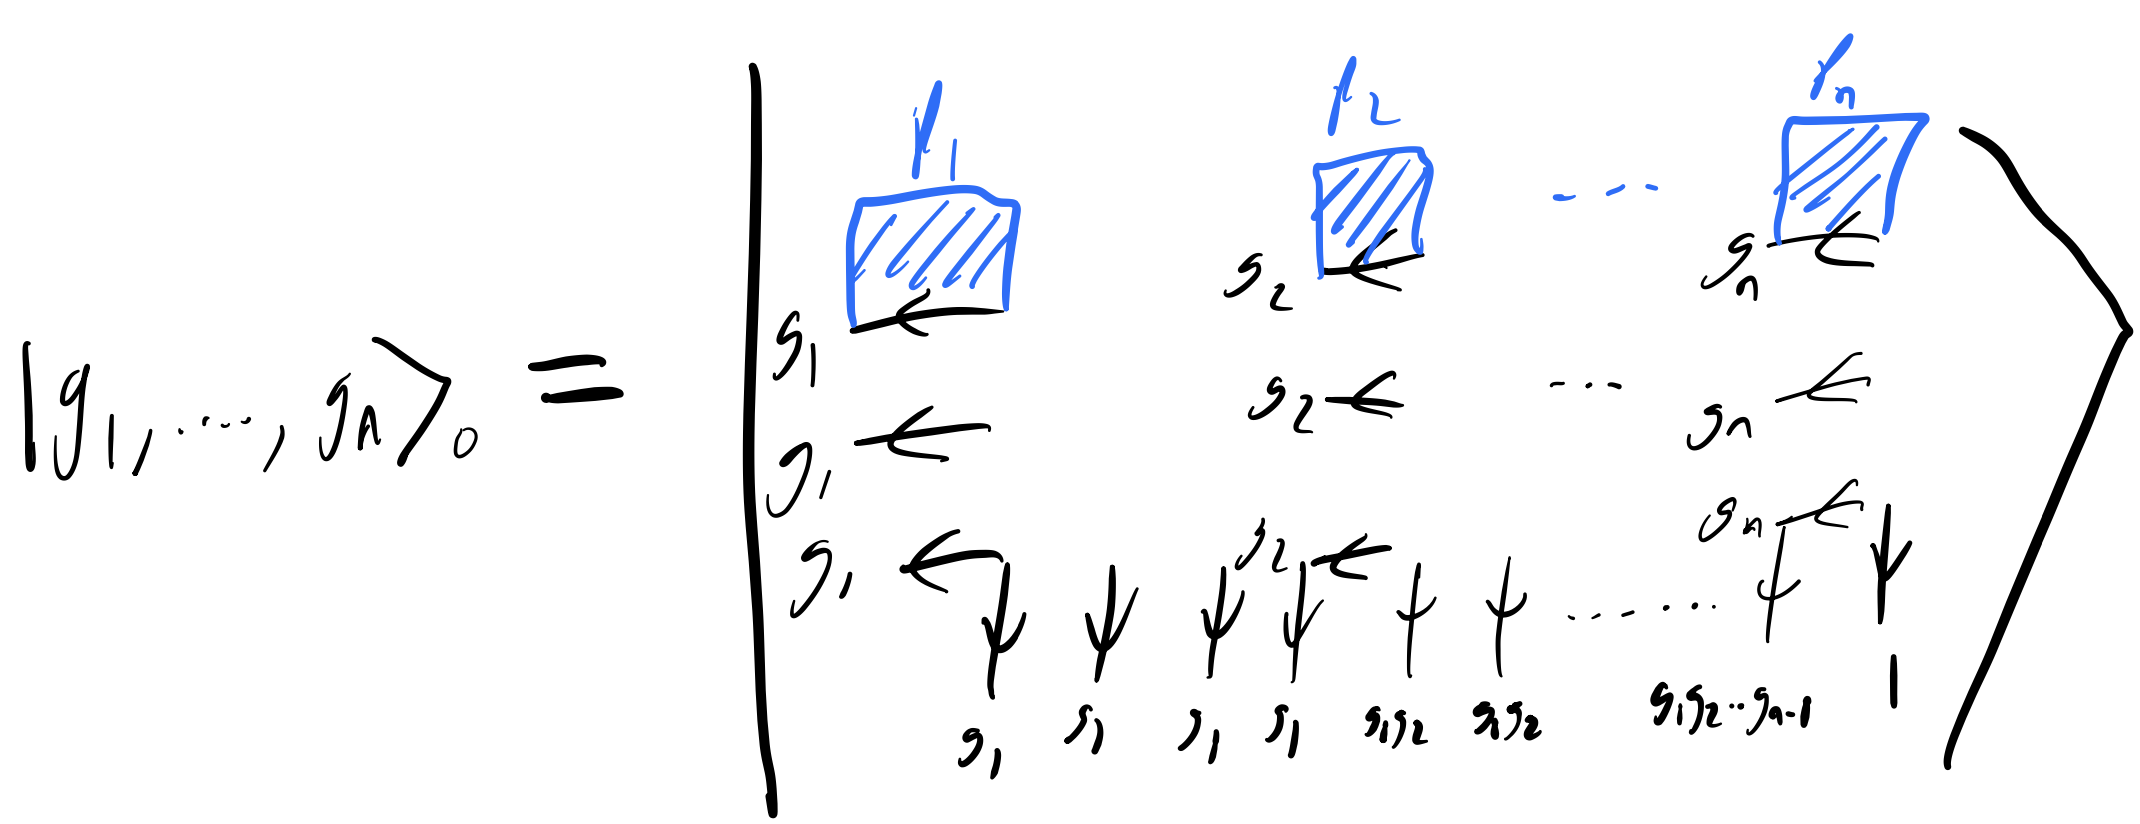
\includegraphics[scale=0.35]{Lectures/Images/lec9-naughtstates.png}
\end{center}
which produces the fluxes at the desired locations, and then we have branch cuts of non-trivial group elements on links such that all other fluxes are trivial ($g_i$ on the vertical columns, and then $g_1 \ldots g_{i-1}$ on the horizontal sections).

By construction, the flux through each $p_i$ is $g_i \in C_i$:
\begin{equation}
    B_c(p_i)\ket{g_1, \ldots g_n}_0 = \ket{g_1, \ldots g_n}_0
\end{equation}
and the flux through all other plaquettes is also 1:
\begin{equation}
    B(p)\ket{g_1, \ldots g_n}_0 = \ket{g_1, \ldots g_n}_0 \quad p \neq p_1, \ldots p_n
\end{equation}
So, so far the plaquette operators likes this state. But the star operators may not. We define the actual ground state to be:
\begin{equation}
    \ket{g_1, \ldots g_n} = \prod_s A(s)\ket{g_1, \ldots g_n}_0
\end{equation}
which is the projection to the $(s) = 1$ subspace. To get a flavour for what the projection does, we remember the definition of $A(s)$ as a sum of $A_g(s)$s; so:
\begin{equation}
    \ket{g_1, \ldots, g_n} = \prod_s\left(\frac{1}{\abs{G}}\sum_g A_g(s)\right)\ket{g_1, \ldots g_n}_0
\end{equation}
So it sums over all possible configurations that can be obtained by $\ket{g_1, \ldots g_n}_0$ via $A_g(s)$s. Because we have now projected into the $A(s) = 1$ subspace (note; there is no fear that the $A(s)$ could destroy the state, because they only have positive matrix elements), by construction these states will be eigenstates of $A(s)$:
\begin{equation}
    A(s)\ket{g_1, \ldots g_n} = \ket{g_1, \ldots, g_n}
\end{equation}
and because all of the terms in the Hamiltonian commute, the fact that these are still eigenstates of the $B$ operators does not change:
\begin{equation}
    B(p)\ket{g_1, \ldots g_n} = \ket{g_1, \ldots g_n} \quad p \neq p_1, \ldots p_n
\end{equation}
\begin{equation}
    B_{C_i}(p_i)\ket{g_1, \ldots g_n} = \ket{g_1, \ldots g_n}
\end{equation}
so indeed, $\ket{g_1, \ldots g_n}$ are eigenstates of every operator in $H$ with eigenvalue $+1$, so these are indeed ground states of $H$.

A side note; we could write the initial state $\ket{C}$ in this language, just imagining that the cut of non-trivial edges goes off to $\infty$.

\subsection{Ground states - redundancy and completeness}
So, we've found some ground states. But these states are actually not all distinct, there is some redundancy. This is because:
\begin{equation}
    \ket{g_1, g_2, \ldots, g_n} = \ket{hg_1h^{-1}, hg_2h^{-1}, \ldots, hg_nh^{-1}}.
\end{equation}
To see this, we note that the $\ket{g_1, g_2, \ldots, g_n}_0$ states are related by a uniform gauge transformation.
\begin{equation}
    \prod_s A_h(s)\ket{g_1, g_2, \ldots, g_n}_0 = \ket{hg_1h^{-1}, hg_2h^{-1}, \ldots, hg_nh^{-1}}_0
\end{equation}
This is evident from looking at the pictorial definition of the $\ket{g_1, g_2, \ldots, g_n}_0$ states. Indeed, every link gets conjugated by $h$:

\begin{center}
    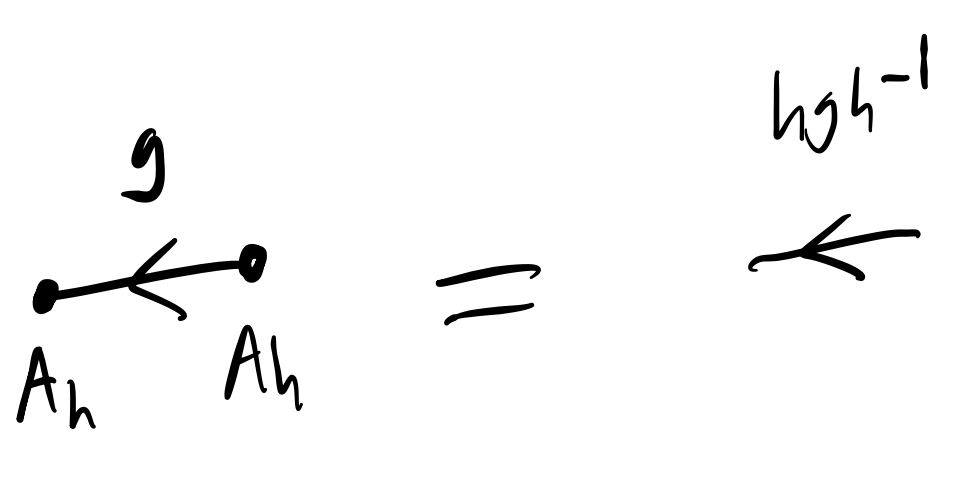
\includegraphics[scale=0.35]{Lectures/Images/lec9-gauging.png}
\end{center}

Because the unprojected states are related by a gauge transformation , when we project onto all the $A(s)$s (and sum over all gauge equivalent combinations) we get the same answer. To see this formally:
\begin{equation}
    \begin{split}
        \ket{hg_1h^{-1}, hg_2h^{-1}, \ldots, hg_nh^{-1}} &= \prod_s\left(\frac{1}{\abs{G}}\sum_g A_g(s)\right)\ket{hg_1h^{-1}, hg_2h^{-1}, \ldots, hg_nh^{-1}}_0
        \\ &= \prod_s\left(\frac{1}{\abs{G}}\sum_g A_g(s)\right)\prod_{s}A_h(s) \ket{g_1, g_2, \ldots, g_n}_0
        \\ &= \prod_{s}\left(\frac{1}{\abs{G}}\sum_g A_g(s)A_h(s) \right)\ket{g_1, g_2, \ldots, g_n}_0
        \\ &= \prod_{s}\left(\frac{1}{\abs{G}}\sum_g A_{gh}(s) \right)\ket{g_1, g_2, \ldots, g_n}_0
        \\ &= \prod_s \left(\frac{1}{\abs{G}}\sum_g A_g(s)\right)\ket{g_1, \ldots, g_n}_0
        \\ &= \ket{g_1, \ldots g_n}
    \end{split}
\end{equation}
where we have used that the group maps to itself under multiplication in the second to last step.

It is not hard to see that this is the only redundancy. Thus:
\begin{equation}
    \braket{g_1, \ldots, g_n}{g_1', \ldots g_n'} = \delta_{g_i' = hg_i h^{-1} \forall i} \quad \text{for some $h \in G$}
\end{equation}
The intuition is that only a uniform gauge transformation can map between the different $\ket{g_1, g_2, \ldots, g_n}_0$ states (else, we get a mismatch on the trivial links, no longer making them trivial). The ground states are sums over gauge configurations, and as such the gauge orbits of non-gauge equivalent $\ket{g_1, g_2, \ldots, g_n}_0$ must be non-overlapping and hence orthogonal.

The punchline: There is a distinct ground state for every $(g_1, \ldots, g_n)$ (ordered list) with $g_1g_2\ldots g_n = 1$ (allowing this state to be created locally), modulo uniform conjugation.

The next question we can ask is - are these all of the ground states? The answer is yes, at least in a sense. These are all the ground states that can be created from $\ket{\Omega}$ (the GS of the original QD model) via an operator acting in a finite region, i.e. around $p_1, \ldots p_n$. It should be clear that we can create these states locally, the converse (that these states consist of all such states) has not been shown explicitly, but is true. In other words, these are the full set of all ground states with trivial ``total topological charge''.

\subsection{Ground state properties}
We label distinct $\ket{g_1, \ldots g_n}$ states by:
\begin{equation}
    \set{\ket{\alpha}, \alpha = 1, \ldots D}
\end{equation}
\begin{enumerate}
    \item There is an exponentially large ground state degeneracy if conjugacy classes have more than one element. For example take $G = S_3 = \set{\II, (12), (13), (23), (123), (132)}$. We have three conjugacy classes:
    \begin{equation}
        C_1 = \set{\II}, \quad C_2 = \set{(12), (13), (23)}, \quad C_3 = \set{(123), (132)}
    \end{equation}
    For $C_2$, we have:
    \begin{equation}
        D_n = \frac{3^{n-1} + 3}{6}
    \end{equation}
    with $n$ - the number of fluxes - here even (you can verify that for $C_2$, no odd number of fluxes can multiply to the identity, as we require).

    More generally, if all $C_i = C$, then:
    \begin{equation}
        D_n \sim \abs{C}^n \cdot \text{const.} \text{ as $n \to \infty$}
    \end{equation}

    \item The ground states are locally indistinguishable. For any $O$ supported on less than $L$ sites where $L = \min_{i, j} \text{dist}(p_i, p_j)$, then:
    \begin{equation}
        \bra{\alpha}O\ket{\beta} = c\delta_{\alpha\beta}
    \end{equation}
    Suppose we have $\ket{g_1, \ldots, g_n}, \ket{g_1', \ldots, g_n'}$. So we might say that there is the ability to distinguish at $p_1$. But for any given flux, I can via conjugation make the flux at $g_1$ look the same $g_1' \to h g_1' h^{-1} = g_1$. So, we need to be able to see more than one flux.

    \item The ground state degeneracy is robust to small local perturbations of $H$. If we take $H \to H + \lambda V$, the splitting is $\delta \sim e^{-\text{const.}L}$. Roughly (as in the toric code case) it follows from property 2, where we need order $L$ perturbation theory to connect states in the ground space.
\end{enumerate}

One last comment - we see the above features, and these are all generic/defining features of non-abelian anyons. Next time, we will look more closely at the non-Abelian nature of these objects, and braid the non-Abelian anyons and look at their braid matrices.